\documentclass{beamer}
\usepackage{graphicx}
\graphicspath{{graphics/}}
\usepackage{caption}
\setbeamertemplate{caption}[numbered]

\usetheme{Warsaw}

\title{Deep Learning - Practical Methodology}

\author{Cosmin G. Alexandru}
\institute{BucharestCV}
\date{March 19, 2017}

\begin{document}

\begin{frame}
\titlepage
\end{frame}

\AtBeginSection[]
{
  \begin{frame}<beamer>
  \frametitle{Layout}
  \tableofcontents[currentsection,currentsubsection]
  \end{frame}
}

\AtBeginSubsection[]
{
  \begin{frame}<beamer>
  \frametitle{Layout}
  \tableofcontents[currentsection,currentsubsection]
  \end{frame}
}

\section{Introduction}\label{sec:introduction}
\begin{frame}
    \frametitle{Introduction}
    Recomended design process:
    \begin{itemize}
        \item Determine your goal - choose performance(error) metric and a target
            for it.
        \item Establish working end-to-end pipeline as soon as possible.
        \item Instrument the system well.
        \item Do incremental changes.
    \end{itemize}
\end{frame}

\section{Performance Metric}\label{sec:perf-metrics}
\begin{frame}
    \frametitle{Peformance Metric}
    \begin{itemize}
        \item Choose a performance metric specific to the problem.
        \item How to determine the target performance:
            \begin{itemize}
                \item Academic setting - Usually, an estimate exists.
                \item Real-world setting - Cost effective, appeal to the customer,
                    usage safety.
            \end{itemize}
        \item Different from the cost function used to train the model.
    \end{itemize}
\end{frame}

\begin{frame}
    \frametitle{Peformance Metric - Examples}
    Performance/error metric examples:
    \begin{itemize}
       \item accuracy
       \item precision and recall
       \item coverage
       \item precision-recall curve
       \item $F-score = \frac{2pr}{p+r}$
       \item $logloss = \frac{-1}{N} $$\sum_{i=1}^{N}$$ $$\sum_{j=1}^{M}$$
           y_{ij}log(p_{ij})$
    \end{itemize}
\end{frame}

\section{Baseline Models}\label{sec:baseline-model}
\begin{frame}
    \frametitle{Baseline Models - Algorithms}
    Baseline algorithms recomandation:
    \begin{itemize}
        \item Simple problem - simple algorithm (e.g. logistic regerssion)
        \item Supervized learning + fixed size input vectors = a feed forword
            network with fully connected layers.
        \item Input with topological structure = convolutional neural network +
            piecewise linear units e.g.: ReLU, Leaky ReLU, PreLus, maxout.
        \item Input or output is a squence = gated recurrent network (LSTM or GRU).
    \end{itemize}
\end{frame}

\begin{frame}
    \frametitle{Baseline Models - Optimization}
    Optimization algorithms:
    \begin{itemize}
        \item Stochastic Gradient Descent(SGD) with momentum.
        \item Adam.\cite{DBLP:journals/corr/KingmaB14}
    \end{itemize}
\end{frame}

\begin{frame}
    \frametitle{Baseline Models - Tips}
    Tips for improving optimization:
    \begin{itemize}
        \item Popular learning rate decay schemes for SGD:
            \begin{itemize}
                \item Linear decay until fixed minimum.
                \item Exponential decay.
                \item Decrease learning rate by a factor of 2-10 each time 
                    validation error plateaus.
            \end{itemize}
        \item Batch normalization can be omitted at first but it should be
            introduced when optimization becomes problematic. It allows for higher
            learning rates.
        \item Dropout is an excellent regularizer.
        \item "Early stoping should be used almost universally."
            \cite{goodfellow-et-al-2016}
    \end{itemize}
\end{frame}

\begin{frame}
    \frametitle{Baseline Models - Supervised vs. Unsupervised}
    Supervised vs. unsupervised learning:
    \begin{itemize}
        \item Start with supervised learning. If the model overfits you can try
            unsupervised learning.
        \item Use unsupervised for applications in a context that is known to
            benefit from unsupervised learning (e.g: natural language processing)
            or the problem you try to solve is unsupervised.
    \end{itemize}
\end{frame}

\section{More Data}\label{sec:more-data}
\begin{frame}
    \frametitle{More Data(0)}
    It is usually better to gather more data than to improve the algorithm. \\~\\

    First check the training set error. High error probably means that the model is
    not using the data.
    Things to try:
    \begin{itemize}
        \item Increase the model size(e.g: number of neurons per layer, number of layers,
            etc.)
        \item Tune the learning rate.
        \item Check the data quality.
    \end{itemize}
\end{frame}

\begin{frame}
    \frametitle{More Data(1)}
    Check error on a test set.
    \begin{itemize}
        \item Small error - you are set.
        \item High  error - gather more data.
    \end{itemize}

    ~\\ If the cost for gathering more data is high, try:
    \begin{itemize}
        \item Adding drop out.
        \item Adjusting hyperparameters.
    \end{itemize}

    ~\\ Plot performance vs. training data size to determine how much data to
    gather in order to obtain the desired performance.
\end{frame}

\section{Hyperparameters}\label{sec:hyperparameters}
\begin{frame}
    \frametitle{Hyperparameters - Search}
    \begin{itemize}
        \item Manual search:
            \begin{itemize}
                \item Start with the learning rate.
            \end{itemize}
        \item Automatic search:
            \begin{itemize}
                \item Gird
                \item Random
            \end{itemize}
        \item Model based search:
            \begin{itemize}
                \item Spearmint\cite{snoek-et-al-2016}
                \item TPE\cite{bergstar-et-al-2011}
                \item SMAC\cite{hutter-et-al-2011}
            \end{itemize}
    \end{itemize}
\end{frame}

\begin{frame}
    \frametitle{Hyperparameters}
    The primary goal of hyperparameter search is to adjust the effective capacity
    of the model.

~\\ Effective capacity of the model depends on three factors:
\begin{itemize}
    \item Representation capacity of the model (more hidden layers / more units per
        hidden layer = greater representational capacity).
    \item Optimization algortihm to successfully minimize the cost function.
    \item Degree to which the cost function and training procedure regularizes the
        model.
\end{itemize}
\end{frame}

\begin{frame}
    \frametitle{Learning rate vs training error}
    \begin{figure}
        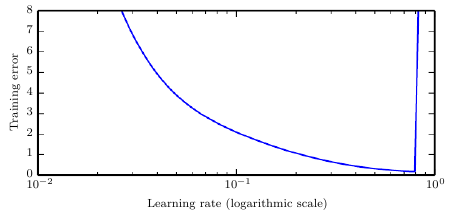
\includegraphics[width=0.85\textwidth]{learn_rate_vs_train_error}
        \caption{Typical relation between learning rate and training error
        (source:\cite{goodfellow-et-al-2016})}
        \centering
    \end{figure}
\end{frame}

\begin{frame}
    \frametitle{What are we searching for}
    Hyperparameter curve:
    \begin{itemize}
        \item Extreme 1: Low capcaity - generalization error high
            because training error is high - underfitting regime.
        \item Extreme 2: High capacity - generalization error is high because
            the gap between the trainging and test error is high - overfitting
            regime
    \end{itemize}

    ~\\ Monitor both train and test error:
    \begin{itemize}
        \item train error higher than target $ \rightarrow $ increase capacity.
        \item tetst error = train error + gap between train error and test error
            (such insight, much wow :P). Goal = reduce gap at a higher rate than
            than the rate at which the training eror increases.
    \end{itemize}
\end{frame}

\begin{frame}
    \frametitle{Grid vs. random search}
    \begin{figure}
        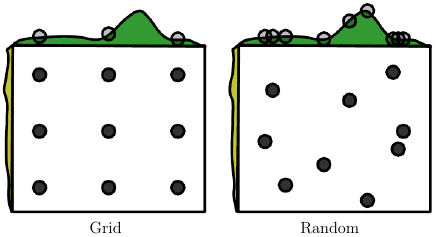
\includegraphics[width=0.75\textwidth]{grid_vs_random_search}
        \caption{Comparison between grid and random search 
        (source:\cite{goodfellow-et-al-2016})}
        \centering
    \end{figure}
\end{frame}

\section{Debugging}\label{sec:debugging}
\begin{frame}
    \frametitle{Debugging}
    Methods to debug software problems:
    \begin{itemize}
        \item Visualize the model in action.
        \item Visualize the worst mistake.
        \item Reason about software using train and test error.
        \item Fit a small dataset.
        \item Compare back-propagation derivatives to numerical derivatives.
        \item Monitor historgrams of activations and gradient.
    \end{itemize}

\end{frame}

\bibliography{practical_methodology}
\bibliographystyle{plain}

\end{document}
